\chapter{四足機器人有限元素分析}

此章節利用了有限元素分析四足機器人,單組步行機構為承受五倍自身重量(630N),材質則選用了常見的ABS材料;分析環境選擇Solid Edge及Ansys同時進行,以利於對比資料並查看兩軟體區別。\\

%-----------------------有限元素分析--------------------------%
\section{有限元素分析}
下列為個部位進行有限元素分析的步驟介紹
\begin{enumerate}
\item 開啟Solid Edge設計模型並執行分析功能新增研究內容 / 另存為IGES(.igs)檔案用以匯入Ansys。
\item 材料選擇3D列印機常用的ABS材質,在未來有能夠快速地打印產出模型。
\item 依照原先設計者的參數設定負載為630N,為自身5倍體重。
\item 通過有限元素法觀察各部位受力狀態。
\item 觀察求解後參數是否符合要求或是需要修改。\

\end{enumerate}
以上步驟為有限元素法在兩個軟體中通過電腦計算在四足機器人上的應用,用兩個軟體分析目的為比較之間的算法差異,以利於後續分析調整。\\

%-----------------------分析比較--------------------------%
\section{Solid Edge與Ansys分析比較}
將零件同時丟進Ansys、Solid Edge進行分析,並比對結果,雖然兩個分析軟體都設定相同的參數,但可能因為軟體的各項因素導致最終結果有所差異,像是軟體使用的模擬方法、網格生成、材料參數、數值設定等因素。\

\begin{enumerate}
\item 分析方式:使用的數值模擬方法和算法可能因為不同的數學模型和近似方法有所差異。
\item 網格生成:使用不同的網格生成算法,導致在相同設定下生成不同的網格。
\item 材料參數:即使設定相同的材料,兩個軟體的數據庫所使用的材料特性和邊界條件等參數也可能有所差異。
\item	數值設定:即使設定相同的參數,兩個軟體可能使用不同的預設值或建議值也會造成差異。\

\end{enumerate}

%-----------------------------------------%
\begin{figure}[hbt!]
\center
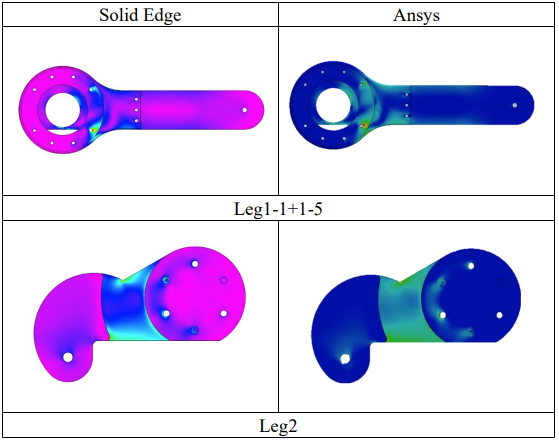
\includegraphics[width=10.5cm]{分析比對表1}
\caption{\Large 分析比對圖}
\label{分析比對表1}
\end{figure}

\begin{figure}[hbt!]
\center
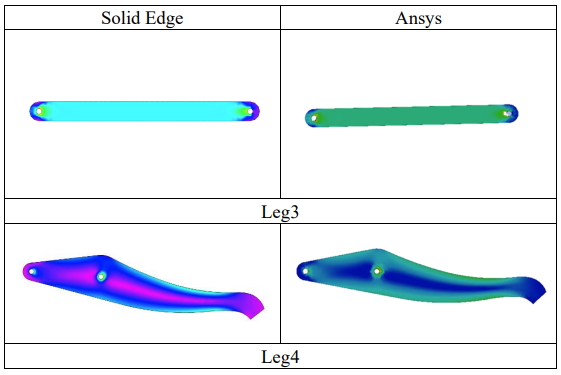
\includegraphics[width=10.5cm]{分析比對表2}
\caption{\Large 分析比對表}
\label{分析比對表2}
\end{figure}

\begin{table}[htb!]
  \center\large
  \setlength{\tabcolsep}{0.75cm}{
  \begin{tabular}{|c|c|c|c|c|}
    \hline &Leg1-1+1-5& Leg2 & Leg3 & Leg4  \\
    \hline Solid Edge &68.5 & 28.9 & 15.8 & 57.6  \\
    \hline Ansys &60.7 & 29.2 & 16.1 & 56.7  \\
    \hline
   \end{tabular}}
  \caption{\Large ABS最大等效應力(MPa)}
\end{table}   

得到分析結果後,發現ABS材料在承受五倍自身體重(630N)時,會導致零件最小安全係數未大於等於1,為了符合實際應用,所以將材料換成強度更高的PLA進行分析。\


\begin{table}[htb!]
  \center
  \large
  \setlength{\tabcolsep}{0.75cm}{
  \begin{tabular}{|c|c|c|c|c|}
    \hline   &Leg1-1+1-5& Leg2 & Leg3 & Leg4 \\
    \hline Solid Edge&69.6 & 30.8 & 15.9 & 61.2  \\
    \hline Ansys &61.2 & 30.0 & 15.8 & 60.5  \\
    \hline
  \end{tabular}}
  \caption{\Large PLA最大等效應力(MPa)}
\end{table}

\begin{table}[htb!]
  \center\large
  \setlength{\tabcolsep}{0.75cm}{
  \begin{tabular}{|c|c|c|c|c|}
    \hline   
    &Leg1-1+1-5& Leg2 & Leg3 & Leg4 \\
    \hline 
    Solid Edge&0.9 & 2.11 & 4.09 & 1.06  \\
    \hline 
    Ansys &1.1 & 2.17 & 4.1 & 1.1  \\
    \hline
  \end{tabular}}
  \caption{\Large PLA最小安全係數}
\end{table}

\newpage
